\documentclass[a4paper]{article}
\usepackage[utf8]{inputenc}
\usepackage{amsmath}
\usepackage{siunitx}
\usepackage[ngerman]{babel}
\usepackage{pgfplots}
\usepackage{hyperref}
\usepackage{pgfplotstable}
\usepackage{csvsimple}
\usepackage[section]{placeins}

\pgfplotsset{compat=1.15}

\title{GPET\\ Auswertung Versuch 2\\ Gruppe 1}

\author{Jonas Otto\\ \href{mailto:jonas@jonasotto.com}{jonas@jonasotto.com} 
   \and Luca Krüger \\ \href{mailto:luca.krueger@uni-ulm.de}{luca.krueger@uni-ulm.de} }
\date{24. April 2018}

\begin{document}

\maketitle

\section{Vorbereitung}

\subsection{Untersuchung eines einfachen Netzwerks}

$U_{R1}=\frac{6}{7}U_{in}$\\
$U_{R2}=U_2=\frac{1}{7}U_{in}$\\
$U_{R3}=U_{R4}=U_1=\frac{1}{14}U_{in}$\\

\noindent
Ersatzspannungsquelle: Spannung $U_{\text{Leerlauf}}=0.214\si{V}$, Kurzschlussstrom  $I_{\text{KS}}=2.5\si{mA}$, Innenwiderstand  $R_{\text{i}}=85.6\si{\ohm}$.

\subsection{Untersuchung eines komplizierten Netzwerks}

\[
\begin{bmatrix}
    5 & -1 & -2 & -1\\
    -1 & 3 & 0 & 0\\
    -2 & 0 & 3 & -1\\
    -1 & 0 & -1 & 3
\end{bmatrix}
\cdot
\begin{bmatrix}
    U_1\\
    U_2\\
    U_3\\
    U_4
\end{bmatrix}
=
\begin{bmatrix}
    0\\
    U_{in1}\\
    U_{in2}\\
    U_{in1}
\end{bmatrix}
\]
$U_1 = \frac{1}{79} (11 \cdot U_{in} + 15)$, 
$U_2 = \frac{5}{79} (6 \cdot U_{in} + 1)$, 
$U_3 = \frac{-3}{79} (U_{in} - 13)$, 
$U_4 = \frac{1}{79} (31 \cdot U_{in} - 8)$

%{5u - v - 2w - x = 0, -u + 3v = y, -2u + 3w + x = 1, -u + w + 3x = y} solve for u,v,w,x
%^so besonders richtig sieht das nicht aus aber es gibt mal ne lösung...


\section{Versuchsauswertung}

\subsection{Bestimmung des Innenwiderstands einer Quelle}
Im folgenden Messaufbau wird die Kennlinie einer Batterie bestimmt. Dafür wurde in Reihe ein variabler Lastwiderstand und ein $50\si{ohm}$ Widerstand an eine $9\si{V}$-Batterie angeschlossen.
Zur Bestimmung der Kennlinie wurde nun der Lastwiderstand verändert und die Spannung der Batterie parallel zu den beiden Widerständen gemessen (Tabelle \ref{tab:messtab1}).
Wir stellen fest, dass die Spannung bei kleinerer Last, also bei größerem Strom, leicht einbricht. Diese Verhalten liegt an dem relativ hohen Innenwiderstand von $75\si{\ohm}$. Die Batterie hat im vollen Zustand einen Innenwidertsand von ca. $3\si{\ohm}$.\\ 
Das bedeutet, dass sich eine Batterie nicht wie eine ideale Spannungsquelle verhält, also der Strom nicht unbegrenzt ist.
%Todo
%Schaltung aufbauen
%Spannung messen, Strom berechnen & in Tabelle Eintragen
\begin{table}[ht]
    \centering
    \begin{tabular}{| c | c | c | c | c | c |}
        \hline
         $R_L [\si{\ohm}]$ & $\infty$ & 1000 & 750 & 500 & 250\\\hline
         $U_{mess} [\si{V}]$ & 8.41 & 7.29 & 7.0 & 6.4 & 5.6\\\hline
         $I_{L} [\si{mA}]$ & 0 & 7.29 & 9.33 & 12.8 & 22.4\\\hline\hline
         $R_L [\si{\ohm}]$ & 200 & 150 & 125 & 100 & 75\\\hline
         $U_{mess} [\si{V}]$ & 5.45 & 5.0 & 4.7 & 4.7 & 4.3\\\hline
         $I_{L} [\si{mA}]$ & 27.45 & 33.3 & 37.6 & 47.0 & 57.3\\\hline
    \end{tabular}
    \caption{Messtabelle für Versuch 1}
    \label{tab:messtab1}
\end{table}

%Diagram zu Aufgabe 3.1
\begin{figure}
    \centering
    \begin{tikzpicture}
    \begin{axis}[
        xlabel={$U_{in} [\si{V}]$},
        ylabel={$[\si{mA}]$},
        xmin=0, xmax=9,
        ymin=0, ymax=50,
        xtick={0,...,9},
        ytick={0,10,...,50},
        legend pos=north west,
        ymajorgrids=true,
        grid style=dashed,
    ]
     
        \addplot[
        color=blue,
        mark=square,
        ]
        coordinates {
        (8.41,0)(7.0,7.29)(7.0,9.33)(6.4,12.8)(5.6,22.4)(5.45,27.45)(5.5,33.3)(4.7,37.6)(4.7,47.0)(4.3,57.3)
        };
        \legend{$\si{U}-\si{I}$-Kennlinie}
    \end{axis}
\end{tikzpicture}
    \caption{Kennlinie der $9\si{V}$-Batterie (Tabelle \ref{tab:messtab1})}
    \label{fig:messtab1_diagramm}
\end{figure}

Aus den Messungen (Tabelle \ref{tab:messtab1}) und Diagramm \ref{fig:messtab1_diagramm} ergibt sich ein angenäherter Innenwiderstand von $75\si{\ohm}$ und eine Leerlaufspannung von $8.41\si{V}$.

\FloatBarrier
\subsection{Untersuchung eines einfachen Netzwerkes}
Das Netzwerk der nächsten Messung besteht aus zwei verschachtelten Spannungsteilern. 
Zunächst wurde unter unterschiedlichen Lasten die abfallende Spannung gemessen und der Strom berechnet. Aus diesen Messergebnissen lässt sich eine Ersatzspannungsquelle aus idealer Spannungsquelle und Innenwiderstand ermitteln.
Der Innenwiderstand ist dabei die Steigung der Kennlinie.
Die äquivalente Ersatzspannungsquelle zum gegebenen Netzwerk hat einen Innenwiderstand von $85.6\si{\ohm}$, eine Leerlaufspannung $U_L=0.214\si{V}$ und einen Kurzschlussstrom  $I_{\text{KS}}=2.5\si{mA}$. Der aus den Messwerten (Tabelle \ref{tab:messtab2_1}) berechnete Innenwiderstand beträgt $~103\si{\ohm}$, wobei die letzten beiden Messwerte wegen starker Abweichung verworfen wurden. Sie sind auf Messfehler zurückzuführen.

Nun wird die abfallende Spannung an jedem Widerstand unter beliebigen Eingangsspannungen gemessen.
Die Messwerte an den einzelnen Widerständen $R_1$ bis $R_4$ (Tabelle \ref{tab:messtab2_2}) stimmen im Allgemeinen mit den berechneten Werten überein (vgl. Abbildungen \ref{fig:u12} und \ref{fig:u34}), bei $U_{R2}$ ist eine Abweichung festzustellen. Da die Messwerte aber sehr genau auf einer Geraden liegen ist anzunehmen, dass der Widerstand einen geringfügig anderen Wert hat, als angegeben.

\begin{table}[ht]
    \centering
    \begin{tabular}{| c | c | c | c | c | c | c | c |}
        \hline
         $R_L [\si{\ohm}]$ & $\infty$ & 1000 & 750 & 500 & 250 & 100 & 50\\\hline
         $U_{mess} [\si{mV}]$ & 223 & 204 & 198 & 186 & 154 & 80 & 1\\\hline
         $I_{L} [\si{mA}]$ & 0 & 0.2 & 0.26 & 0.37 & 0.62 & 0.8 & 0.02\\\hline
    \end{tabular}
    \caption{Messtabelle für Versuch 2}
    \label{tab:messtab2_1}
\end{table}

\begin{table}[ht]
    \centering
    \begin{tabular}{| c | c | c | c | c | c | c | c |}
        \hline
         $U_{in} [\si{V}]$ & 0 & $0.5$ & $1$ & $1.5$ & $2$ & $2.5$ & $3$ \\\hline
         $U_{R1,soll} [\si{V}]$ & 0 & $0.43$ & $0.86$ & $1.29$ & $1.72$ & $2.15$ & $2.58$ \\\hline %Uin-UR2
         $U_{R2,soll} [\si{V}]$ & $0$ & $0.07$ & $0.14$ & $0.21$ & $0.28$ & $0.35$ & $0.42$ \\\hline
         $U_{R3,soll} [\si{V}]$ & 0 & $0.0355$ & $0.071$ & $0.1065$ & $0.142$ & $0.1775$ & $0.213$ \\\hline
         $U_{R3,soll} [\si{V}]$ & 0 & $0.0355$ & $0.071$ & $0.1065$ & $0.142$ & $0.1775$ & $0.213$ \\\hline
         $U_{R1,mess} [\si{V}]$ & 0 & 0.43 & 0.89 & 1.33 & 1.77 & 2.17 & 2.59 \\\hline
         $U_{R2,mess} [\si{V}]$ & 0 & 0.073 & 0.15 & 0.23 & 0.30 & 0.37 & 0.44\\\hline
         $U_{R3,mess} [\si{V}]$ & 0 & 0.037 & 0.077 & 0.12 & 0.16 & 0.19 & 0.23\\\hline
         $U_{R4,mess} [\si{V}]$ & 0 & 0.035 & 0.073 & 0.11 & 0.15 & 0.18 & 0.22 \\\hline
    \end{tabular}
    \caption{Messtabelle für Versuch 2}
    \label{tab:messtab2_2}
\end{table}

\begin{figure}[ht]
    \centering
    \begin{tikzpicture}
    \begin{axis}[
        xlabel={$U_{in} [\si{V}]$},
        ylabel={U [\si{V}]},
        xmin=0, xmax=3,
        ymin=0, ymax=3,
        xtick={0, 1, 2, 3},
        ytick={0, 1, 2, 3},
        legend pos=north west,
        ymajorgrids=true,
        grid style=dashed,
    ]
    \addplot[   %Ur1
        color=red,
        domain=0:3,
        ]
        {x-0.14*x};
    \addplot[
        color=red,
        mark=square,
        ]
        coordinates {
        (0,0)(0.5,0.43)(1,0.89)(1.5,1.33)(2,1.77)(2.5,2.17)(3,2.59)
        };
        
    \addplot[   %Ur2
        color=blue,
        domain=0:3,
        ]
        {0.14*x};
    \addplot[
        color=blue,
        mark=square,
        ]
        coordinates {
        (0,0)(0.5,0.037)(1,0.077)(1.5,0.12)(2,0.16)(2.5,0.19)(3,0.23)
        };
    
    \legend{$U_{R1}$ (Berechnet), $U_{R1}$ (Gemessen), $U_{R2}$ (Berechnet), $U_{R2}$ (Gemessen)}
    \end{axis}
\end{tikzpicture}
    \caption{Spannungen an $R_1$ und $R_2$ (Tabelle \ref{tab:messtab2_2})}
    \label{fig:u12}
\end{figure}

\begin{figure}[ht]
    \centering
    \begin{tikzpicture}
    \begin{axis}[
        xlabel={$U_{in} [\si{V}]$},
        ylabel={U [\si{V}]},
        xmin=0, xmax=3,
        ymin=0, ymax=0.3,
        xtick={0, 1, 2, 3},
        ytick={0, 0.1, 0.2, 0.3},
        legend pos=north west,
        ymajorgrids=true,
        grid style=dashed,
    ]
    \addplot[   %Ur3=Ur4
        color=purple,
        domain=0:3,
        ]
        {0.07*x};
    \addplot[
        color=red,
        mark=square,
        ]
        coordinates {
        (0,0)(0.5,0.037)(1,0.077)(1.5,0.12)(2,0.16)(2.5,0.19)(3,0.23)
        };
    \addplot[
        color=blue,
        mark=square,
        ]
        coordinates {
        (0,0)(0.5,0.035)(1,0.073)(1.5,0.11)(2,0.15)(2.5,0.18)(3,0.22)
        };
    
    \legend{$U_{R3}=U_{R4}$ (Berechnet), $U_{R3}$ (Gemessen), $U_{R4}$ (Gemessen)}
    \end{axis}
\end{tikzpicture}
    \caption{Spannungen an $R_3$ und $R_4$ (Tabelle \ref{tab:messtab2_2})}
    \label{fig:u34}
\end{figure}

\FloatBarrier
\subsection{Untersuchung eines komplizierten Netzwerkes}
Die Messwerte an den einzelnen Knoten sind in Tabelle \ref{tab:messtab3} eingetragen. Im Rahmen von kleinen Messungenauigkeiten stimmen sie mit den Berechnungen aus Matlab (Abbildung \ref{fig:matlabPlot}) überein.

\begin{table}[ht]
    \centering
    \begin{tabular}{| c | c | c | c | c | c | c | c |}
        \hline
         $U_{in,1} [\si{V}]$   & 0     & $0.5$ & $1$   & $1.5$ & $2$   & $2.5$ & $3$   \\\hline
         $U_{1,mess} [\si{V}]$ & 0     & 0.169 & 0.366 & 0.514 & 0.774 & 1.007 & 1.193 \\\hline
         $U_{2,mess} [\si{V}]$ & 0.016 & 0.236 & 0.458 & 0.706 & 0.919 & 1.181 & 1.391 \\\hline
         $U_{3,mess} [\si{V}]$ & 0.346 & 0.573 & 0.807 & 1.063 & 1.286 & 1.557 & 1.776 \\\hline
         $U_{4,mess} [\si{V}]$ & 0.130 & 0.421 & 0.726 & 1.057 & 1.344 & 1.698 & 1.981 \\\hline
    \end{tabular}
    \caption{Messtabelle für Versuch 3}
    \label{tab:messtab3}
\end{table}

\begin{figure}[ht]
    \caption{Matlab Plot der Knotenpotentialanalyse zu Aufgabe 3}
    \centering
    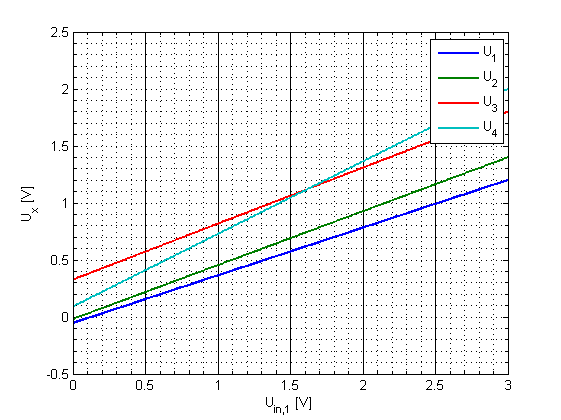
\includegraphics[width=0.7\textwidth]{matlabPlot.png}
    \label{fig:matlabPlot}
\end{figure}

\FloatBarrier
\subsection{Wheatstone Messbrücke}

Nach Aufbau der Messbrücke wurden nacheinander Widerstände mit den Werten $220\si{\ohm}$, $100\si{\ohm}$, $680\si{\ohm}$ eingesetzt.
Nach dem Abgleichen der Messbrücke, dass $U_{21}=0\si{V}$ beträgt, lässt sich der Widerstand durch $R_x=\frac{R_3 R_1}{R_2}$ berechnen (Tabelle \ref{tab:wsbridge}).
Ist der zu messende Widerstand kleiner als $R_1=100\si{\ohm}$, kann die Messbrücke nicht mehr abgeglichen werden, da mit dem Potentiometer $R_2$ nicht mehr als $1\si{k\ohm}$ eingestellt und damit nicht das gleiche Verhältnis erreicht werden kann.
Das größtmögliche Verhältnis $\frac{R_2}{R_3}$ ist $1$. Um dennoch kleine Widerstände zu messen, kann entweder $R_1$ oder $R_3$ verkleinert werden oder ein Potentiometer mit größerem maximalen Widerstand an Stelle $R_2$ gewählt werden.
Auch wenn der zu messende Widerstand sehr groß ist kann er nicht mehr gemessen werden, da das Ablesen des Wertes am Potentiometer nicht mehr möglich ist. Um dies zu verhindern kann der Widerstand in Reihe mit dem zu Messenden vergrößert werden.
In Tabelle \ref{tab:wsbridge} sind die Messwerte eingetragen. Die Abweichung vom erwarteten Wert erklärt sich durch Toleranz der Widerstände und kleine Ungenauigkeit beim Ablesen vom Potentiometer.
\begin{table}[ht]
    \centering
    \begin{tabular}{c|c}
         Erwarteter Wert & Gemessener Wert \\\hline
         $220\si{\ohm}$ & $219.7\si{\ohm}$\\
         $100\si{\ohm}$ & $101\si{\ohm}$\\
         $680\si{\ohm}$ & $666\si{\ohm}$
    \end{tabular}
    \caption{Messungen verschiedener Widerstände mittels Wheatstone Brücke}
    \label{tab:wsbridge}
\end{table}
\end{document}